\documentclass[a4paper,regno]{article}
\usepackage[slovene]{babel}
\usepackage[utf8]{inputenc}
\usepackage[T1]{fontenc}
\usepackage{amsmath}
\usepackage{graphicx}
\usepackage{lmodern}
\usepackage{amsfonts}
\usepackage{amsthm}
\usepackage{float}
\usepackage{}

%\pagestyle{fancy}
%\fancyhf{}


% Definicija okolij izrek, posledica
{\theoremstyle{plain}
\newtheorem{izrek}{Izrek}%[section]
\newtheorem{lema}[izrek]{Lema}
}
% Definicija okoli za definicije in vaje
{\theoremstyle{definition}
\newtheorem{definicija}[izrek]{Definicija}
\newtheorem{vaja}[izrek]{Vaja}
}


\usepackage{subfig}
\usepackage{graphicx}
\graphicspath{{./slike/}}


\title{Gregoryjeve krpe\\
\Large Seminarska naloga pri predmetu RPGO}

\date{}
\author{Klara Kresnik in Meta Trdin\\
%2. letnik\\
Fakulteta za matematiko in fiziko\\
}

%\address{Fakulteta za matematiko in fiziko}

\newcounter{definicija}
\newcommand{\tbf}{\textbf}

%\newenvironment{definicija}
%{
%	\refstepcounter{definicija}
%	\begin{flushleft}
%		\textbf{Definicija \arabic{definicija}:}
%}{
%	%\hfill $\square$ ta hfill sam nardi presledek pred definicijo
%	\end{flushleft} 
%}

%poišči kako se poravna besedilo
%naj bo prva stran cela samo naslov in zacni na drugi strani

\begin{document}
\maketitle
% še kera fakulteta
%predmet seminar
%drugi letnik
% \pagebreak



\section{Uvod}
%presdtavitev problema
Za začetek najprej predstavimo problem. Krpe oziroma ploskve v prostoru želimo zlepiti tako, da bo vzdolž skupnega roba dosežena geometrijska zveznost reda 1. To bomo lahko dosegli lokalno. Zaradi lokalne $G^1$ zveznosti se Gregoryjeve krpe uporablja pri geometrijskem modeliranju in v računalniški grafiki. S predavanj vemo, da nam $G^1$ zveznost zagotavlja zveznost enotskih tangent, kar v našem primeru pomeni, da se morata tangentni ravnini ene in druge krpe ujemati.

Ko združujemo dve krpi, naletimo na problem. Reče se mu twist compatibility problem ali tudi vertex inconsistency problem in sicer ni nujno, da bodo mešani odvodi enaki.
Kot vemo se pri polinomski konstrukciji mešani odvodi ujemajo, v primeru Gregoryjevih krp pa niti ni treba, da se (glej sliko \ref{fig:mesani odvodi}). To je tudi ena izmed prednosti. Pokaže se pri računanju notranjih kontrolnih točk, kjer bo posamezna točka postala racionalna funkcija, zato bo ploskev sama po sebi racionalna.

\begin{figure}[h]
	\centering
	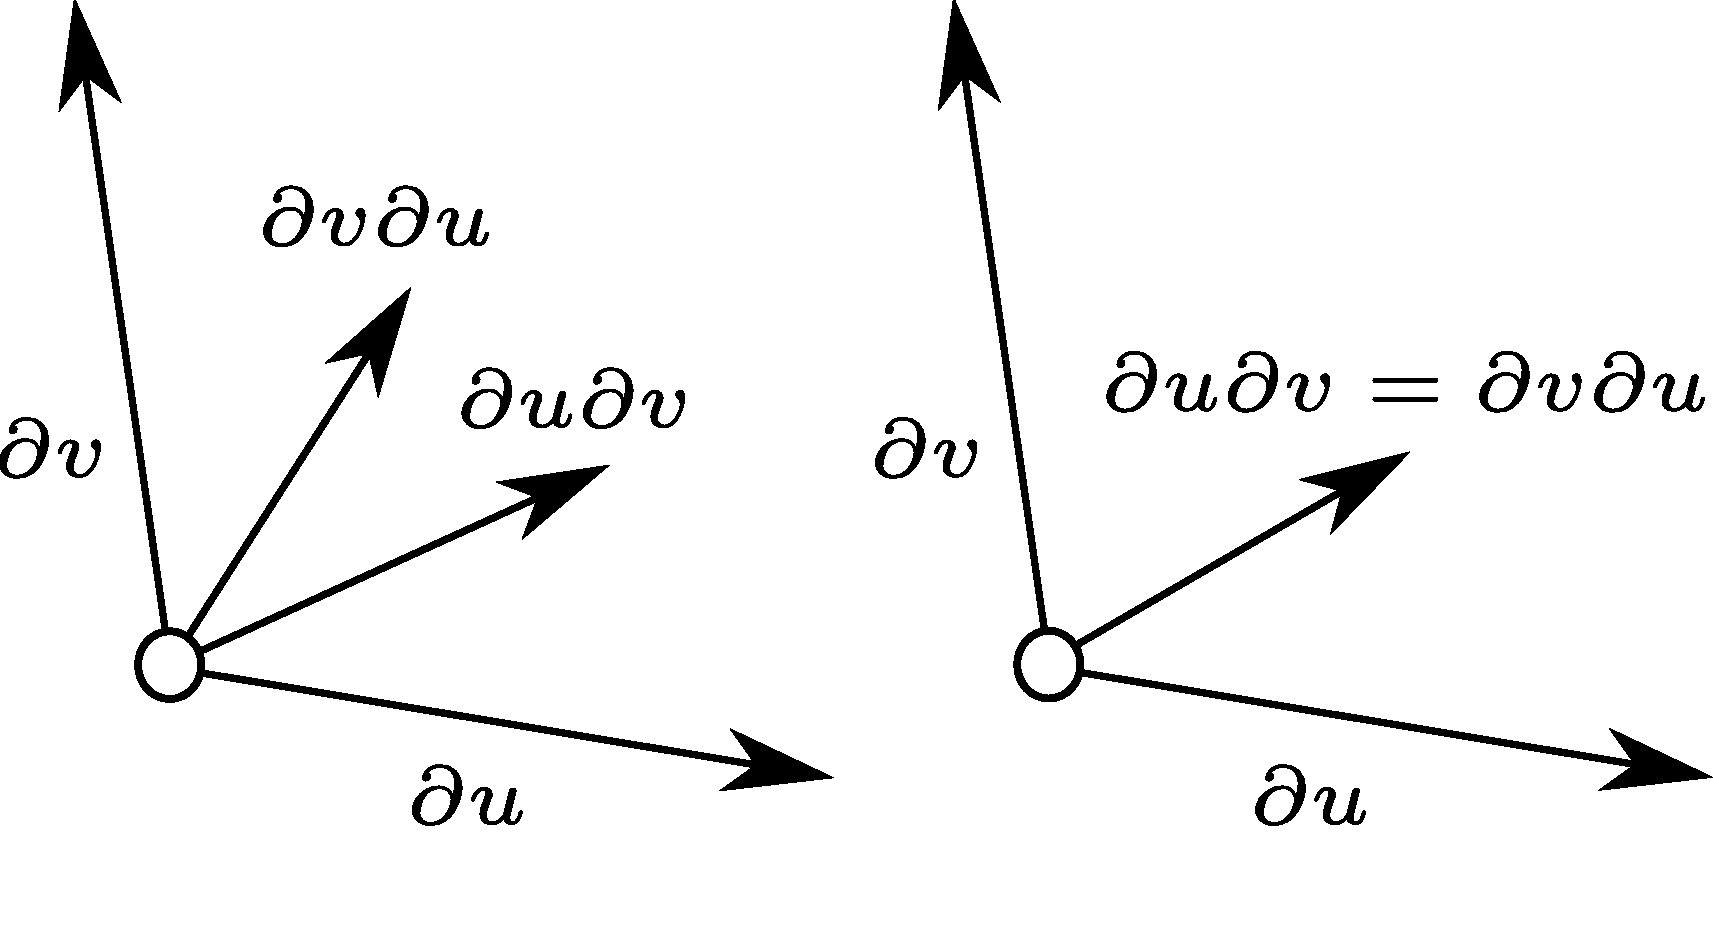
\includegraphics[width=7cm]{mesani_odvodi_ob.jpg}
	\caption{Levo: mešani odvodi v primeru Gregoryjeve krpe; Desno: mešani odvodi pri polinomski konstrukciji}
	\label{fig:mesani odvodi}
\end{figure}

Podane bomo imeli robne krivulje, ki bodo kar Bézierjeve krivulje stopnje $3$. Računali 
bomo notranje kontrolne točke. Pri tem bomo potrebovali tudi podatke s tangentne ravnine 
na robu, da bomo lahko zagotovili $G^1$ zveznost. To nas pripelje do metode Chiyokura in 
Kimura. 


\section{Metoda Chiyokura in Kimura}
	Metoda združi dve Bézierjevi ploski, tako da imamo na skupnem robu G$^1$ zveznost.
	Kot vhodne podatke bomo imeli na voljo samo podatke o skupnem robu in vektorjih iz
	tangentne ravnine. V izhodu nam metoda poda notranje točke ploskve. Zaradi lokalnosti 
	podatkov bo zlepek zgolj lokalno G$^1$ zvezen.
	
	Za primer bomo metodo aplicirali na dveh Bézierjevih ploskvah iz tenzorskega produkta 
	stopnje 3, $\Phi_a$ in $\Phi_b$. Metoda nam vrne notranji točki na ploskvi 
	$\Phi_a$ (slika \ref{fig:domenski_kvadrat_chi_ki}). To ploskev poimenujemo osnovna 
	ploskev in ploskev $\Phi_b$ pridružena ploskev. Da dobimo G$^1$ zveznost na robu, 
	moramo izračunati tudi notranji točki na ploskvi $\Phi_b$. To naredimo tako, da ploskev 
	$\Phi_b$ vzamemo za osnonvo ploskev in ploskev $\Phi_a$ za pridruženo.

	\begin{figure}[h]
		\centering
		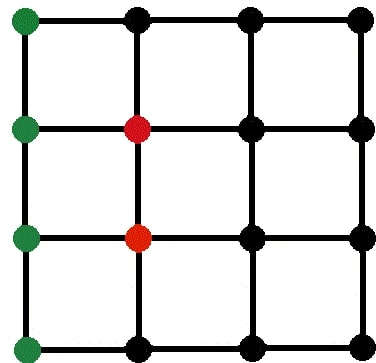
\includegraphics[width=5cm]{kvadratna_domena.jpg}
		\caption{Kontrolne točke Bézierjeve ploskve iz tenzorskega produkta stopnje 3. Zelene točke so
		kontrolne točke krivulje na skupnem robu. Rdeči točki 
		sta kontrolni točki, ki ju dobimo z izvedbo metode Chiyokura in Kimura.}
		\label{fig:domenski_kvadrat_chi_ki}
	\end{figure}

	G$^1$ zveznost lahko karakteriziramo s tangentnimi vektorji.
	Definirajmo krivuljo $\Gamma(u)$, ki za parametre $u \in [0, 1]$, parametrizira 
	krivuljo na skupnem robu zlekpa. Tangentni vektor te krivulje označimo z 
	$\partial \Gamma(u)$. Tangentni vektor ploskve $\Phi_a$, ki je pravokoten na vektor
	$\partial \Gamma(u)$ označimo z $\partial \Gamma_a(u)$ in na podoben način definiramo
	vektor $\partial \Gamma_b(u)$. Zlepek bo G$^1$ zvezen natanko takrat, ko bodo 
	vektorji $\partial \Gamma(u)$, $\partial \Gamma_a(u)$ in $\partial \Gamma_b(u)$
	koplanarni, oziroma, ko velja 
	\begin{equation}
		\label{eq:det}
		\text{det} (\partial \Gamma(u), \partial \Gamma_a(u), \partial \Gamma_b(u)) = 0, \ u \in [0, 1]
	\end{equation}
	
	Na sliki \ref{fig:chi_ki_metoda} so z modro obarvani vhodni podatki.
	Točke obarvane z zeleno in rdečo se ujemajo z obarvanimi točkami na sliki 
	\ref{fig:domenski_kvadrat_chi_ki}, torej je naš cilj izračunati vektorja $\textbf{a}_1$ in 
	$\textbf{a}_2$.  Namesto kontrolnih točk imamo podane vektorje. Vektorji $\textbf{c}_0, \textbf{c}_1$ in $\textbf{c}_2$
	definirajo kontrolne točke za krivuljo na skupnem robu. Vektorja $\textbf{a}_0$ in $\textbf{a}_3$ 
	sta tangenta na ploskev $\Phi_a$ in podobno sta vektorja $\textbf{b}_0$ in $\textbf{b}_3$ tangenta 
	na ploskev $\Phi_b$. Poleg tega morata slednja biti enotska,
	vsak posebej pravokoten na $\textbf{c}_0$ in $\textbf{c}_2$ in ležati v ravnini katere normala je določena
	v ogljiščih $v_i$ in $v_{i + 1}$.

	Da bomo lahko izračunali vektorja $\textbf{a}_1$ in $\textbf{a}_2$ zapišimo enačbo, ekvivalentno
	enačbi \ref{eq:det}, s pomočjo skalarnih funkcij $k(u)$ in $h(u)$:

	\begin{equation}
		\label{eq:k in h}
		\partial \Gamma_a(u) = k(u) \partial \Gamma_b(u) + h(u) \partial \Gamma(u)
	\end{equation}
	
	Da rešimo enačbo \ref{eq:k in h}, izrazimo $a_0$ in $a_3$
	\begin{equation*}
		\begin{split}
			\tbf{a}_0 &= k_0\tbf{b}_0 + h_0\tbf{c}_0 \\
		\end{split}
		\quad\quad
		\begin{split}
			\tbf{a}_3 &= k_1\tbf{b}_3 + h_1\tbf{c}_2 \\
		\end{split}
	\end{equation*},
	kjer so $k_0, k_1, h_0, h_1 \in \mathbb{R}$. Sledi, da sta iskani funkciji
	\begin{equation*}
		\begin{split}
			k(u) &= (1 - u) k_0 + u k_1 \\
		\end{split}
		\quad\quad
		\begin{split}
			h(u) &= (1 - u) h_0 + u h_1 \\
		\end{split}
	\end{equation*}

	Vektorja $\textbf{b}_1$ in $\textbf{b}_2$ določimo z linearno interpolacijo 
	vektorjev $\textbf{b}_0$ in $\textbf{b}_3$.

	\begin{equation*}
		\begin{split}
			\tbf{b}_1 &= \frac{2}{3}\tbf{b}_0 + \frac{1}{3}\tbf{b}_3
		\end{split}
		\quad\quad
		\begin{split}
			\tbf{b}_2 &= \frac{1}{3}\tbf{b}_0 + \frac{2}{3}\tbf{b}_3
		\end{split}
	\end{equation*}

	Sedaj imamo vse podatke, da lahko zapišemo enačbi za $\textbf{a}_1$ in $\textbf{a}_2$.

	\begin{align*}
		\tbf{a}_1 &= (k_1 - k_0)\frac{\tbf{b}_0}{3} + k_0\tbf{b}_1 + 2h_0\frac{\tbf{c}_1}{3} + h_1\frac{\tbf{c}_0}{3} \\
		\tbf{a}_2 &= k_1\tbf{b}_2 - (k_1 - k_0)\frac{\tbf{b}_3}{3} + h_0\frac{\tbf{c}_2}{3} + 2h_1\frac{\tbf{c}_1}{3}
	\end{align*}

	\begin{figure}[h]
		\centering
		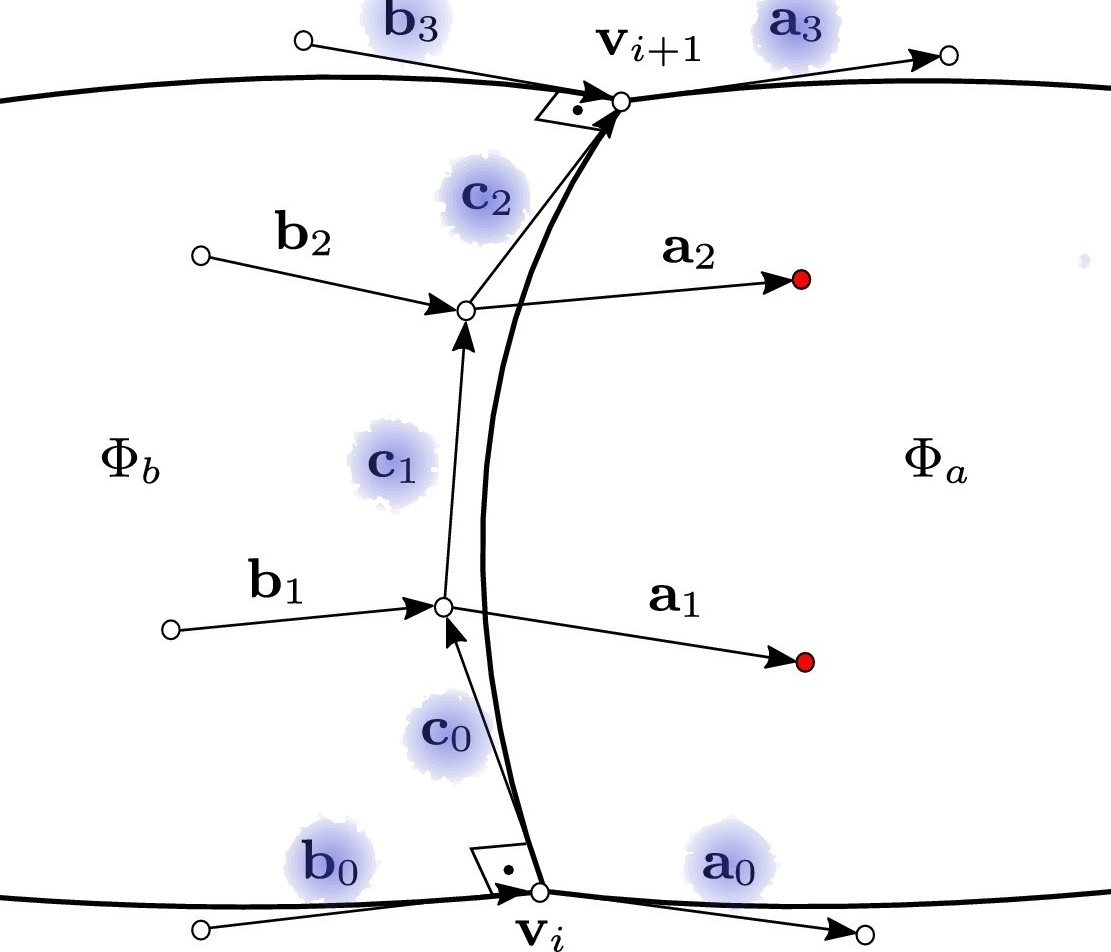
\includegraphics[width=10cm]{metoda_CinK_pobarvano.jpg}
		\caption{Prikaz podatkov pri metodi Chiyokura in Kimura.}
		\label{fig:chi_ki_metoda}
	\end{figure}


\section{Gregoryjeve krpe}
Z Gregoryjevimi krpami posplošimo Gregoryjeve ideje za tenzorski produkt Bézierjevih krp.
Konstruirati želimo ploskev, ki bo imela na robu geometrijsko zveznost reda $1$, ko jo bomo zlepili z drugimi ploskvami, pri tem pa bomo imeli podane le robne krivulje. V nadaljevanju bomo obravnavali trikotne in štirikotne ploskve. Gregoryjeve krpe delamo tudi nad večkotniki višje stopnje, vendar se s tem ne bomo ukvarjali.

Poglejmo si kontrukciji štirikotne in trikotne Gregoryjeve krpe.


\subsection{Kvadratne Gregoryjeve krpe}
Imamo štiri kubične Bézierjeve krivulje, kjer vsaka predstavlja rob Gregoryjeve krpe. Na vsakem robu uporabimo metodo Chiyokura in Kimura in tako pridelamo po $2$ točki. Tako zagotovimo $G^1$ zveznost. Tukaj nastopi twist compatibility problem in sicer dobljene točke ne sovpadajo, kot prikazuje slika \ref{fig:kvadratna}.

\begin{figure}[h]
	\centering
	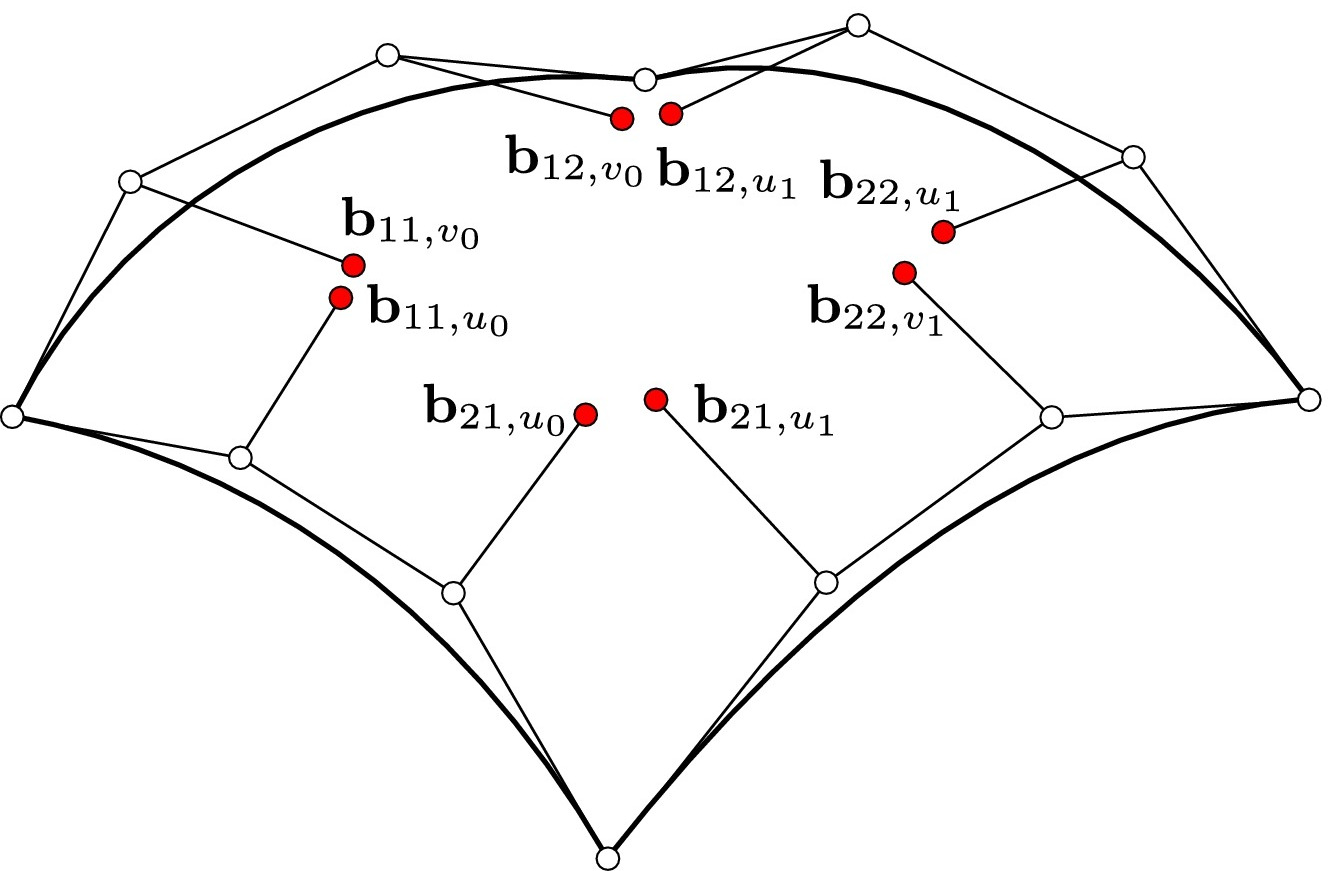
\includegraphics[width=10cm]{gregory_krpe_kvadratna.jpg}
	\caption{Konstrukcija kvadratne Gregoryjeve krpe}
	\label{fig:kvadratna}
\end{figure}

Na tem mestu si pomagamo z racionalnimi funkcijami. Točke $\tbf{b}_{11}, \tbf{b}_{21}, \tbf{b}_{12}, \tbf{b}_{22}$ definiramo kot racionalne funkcije odvisne od parametrov $u$ in $v$ z intervala $[0,1]$:
\begin{align*}
\tbf{b}_{11}(u,v) &=  \frac{v \textbf{b}_{11,u_0}+u\tbf{b}_{11,v_0}}{u +v} \\
\tbf{b}_{21}(u,v) &= \frac{(1-v) \tbf{b}_{21,u_0}+u\tbf{b}_{21,v_1}}{(1-v)+u} \\
\tbf{b}_{12}(u,v) &= \frac{v \tbf{b}_{12,u_1}+(1-u)\tbf{b}_{12,v_0}}{v+(1-u)} \\
\tbf{b}_{22}(u,v) &= \frac{(1-v) \tbf{b}_{22,u_1}+(1-u)\tbf{b}_{22,v_1}}{(1-u)+(1-v)} 
\end{align*}
Če v vsako točko vstavimo določen $(u,v)$ iz roba domene dobimo ravno točke, pridobljene iz metode Chiyokura in Kimura. Opazimo, da se singularnosti v imenovalcu pojavijo le v ogljiščih domene, te pa se da obladati z analizo vrednosti v parametrih.
	

\subsection{Trikotne Gregoryjeve krpe}
Kot že ime pove imamo pri trikotnih Gregoryjevih krpah trikotno domeno, tako da uporabljamo baricentrične koordinate. Imamo $3$ kubične Bézierjeve krivulje na robu, mi pa želimo dobiti notranje kontrolne točke za našo ploskev. Enako kot prej, po metodi Chiyokura in Kimura pridelamo po $2$ točki z vsake stranice.
\begin{figure}[h]
	\centering
	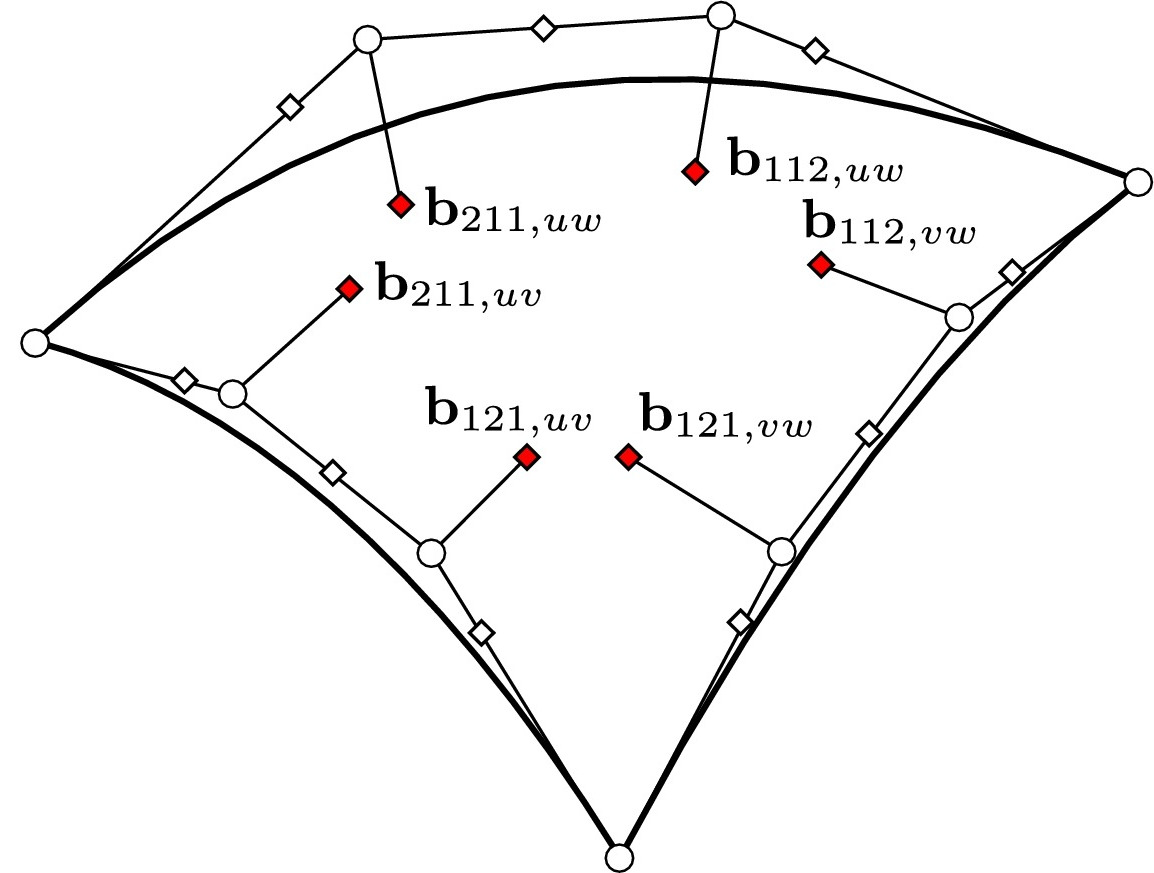
\includegraphics[width=10cm]{gregory_krpe_trikotna.jpg}
	\caption{Konstrukcija trikotne Gregoryjeve krpe}
	\label{fig:trikotna}
\end{figure}

Spet opazimo, da se točke ne ujemajo in tako definiramo racionalne funkcije, ki bodo predstavljale kontrolne točke:
\begin{align*}
\tbf{b}_{211}(u,v,w) &= \frac{(1-w)v \tbf{b}_{211,uv}+(1-v)w\tbf{b}_{211,v_1}}{(1-w)v+(1-v)w} \\
\tbf{b}_{121}(u,v,w) &= \frac{(1-w)u \tbf{b}_{121,uv}+(1-u)v\tbf{b}_{121,vw}}{(1-w)u+(1-u)w} \\
\tbf{b}_{112}(u,v,w) &= \frac{(1-u)v \tbf{b}_{112,vw}+(1-v)u\tbf{b}_{112,uw}}{(1-u)v+(1-v)u} 
\end{align*}

Argumenti o singularnosti so enaki kot prej. Kubična Beziejeva krpa ima le eno notranjo kontrolno točko, za krpo stopnje $4$ pa vemo, da jih ima $3$. V našem primeru nam zato bolj ustreza slednji primer, saj imamo definirane tri različne funkcije za te točke. Robnim krivuljam tako še zvišamo stopnjo, da dobimo mrežo za krpo stopnje $4$. Te točke so na sliki \ref{fig:trikotna} označene kot kare.


\section{Zaključek}
Za konec si poglejmo nekaj primerov. Za prvi primer  sva za osnovo vzeli kocko in nato v programu Matlab na stranicah implementirali $G^1$ zveznost. Dobljeno telo prikazuje slika \ref{fig:g_kocka}. Na sliki se vidijo tudi točke $\tbf{b}_{11}(u,v),
\tbf{b}_{21}(u,v), \tbf{b}_{12}(u,v), \tbf{b}_{22}(u,v)$, ki jih dobimo pri različnih parametrih $u$ in $v$.
\begin{figure}[H]
	\centering
	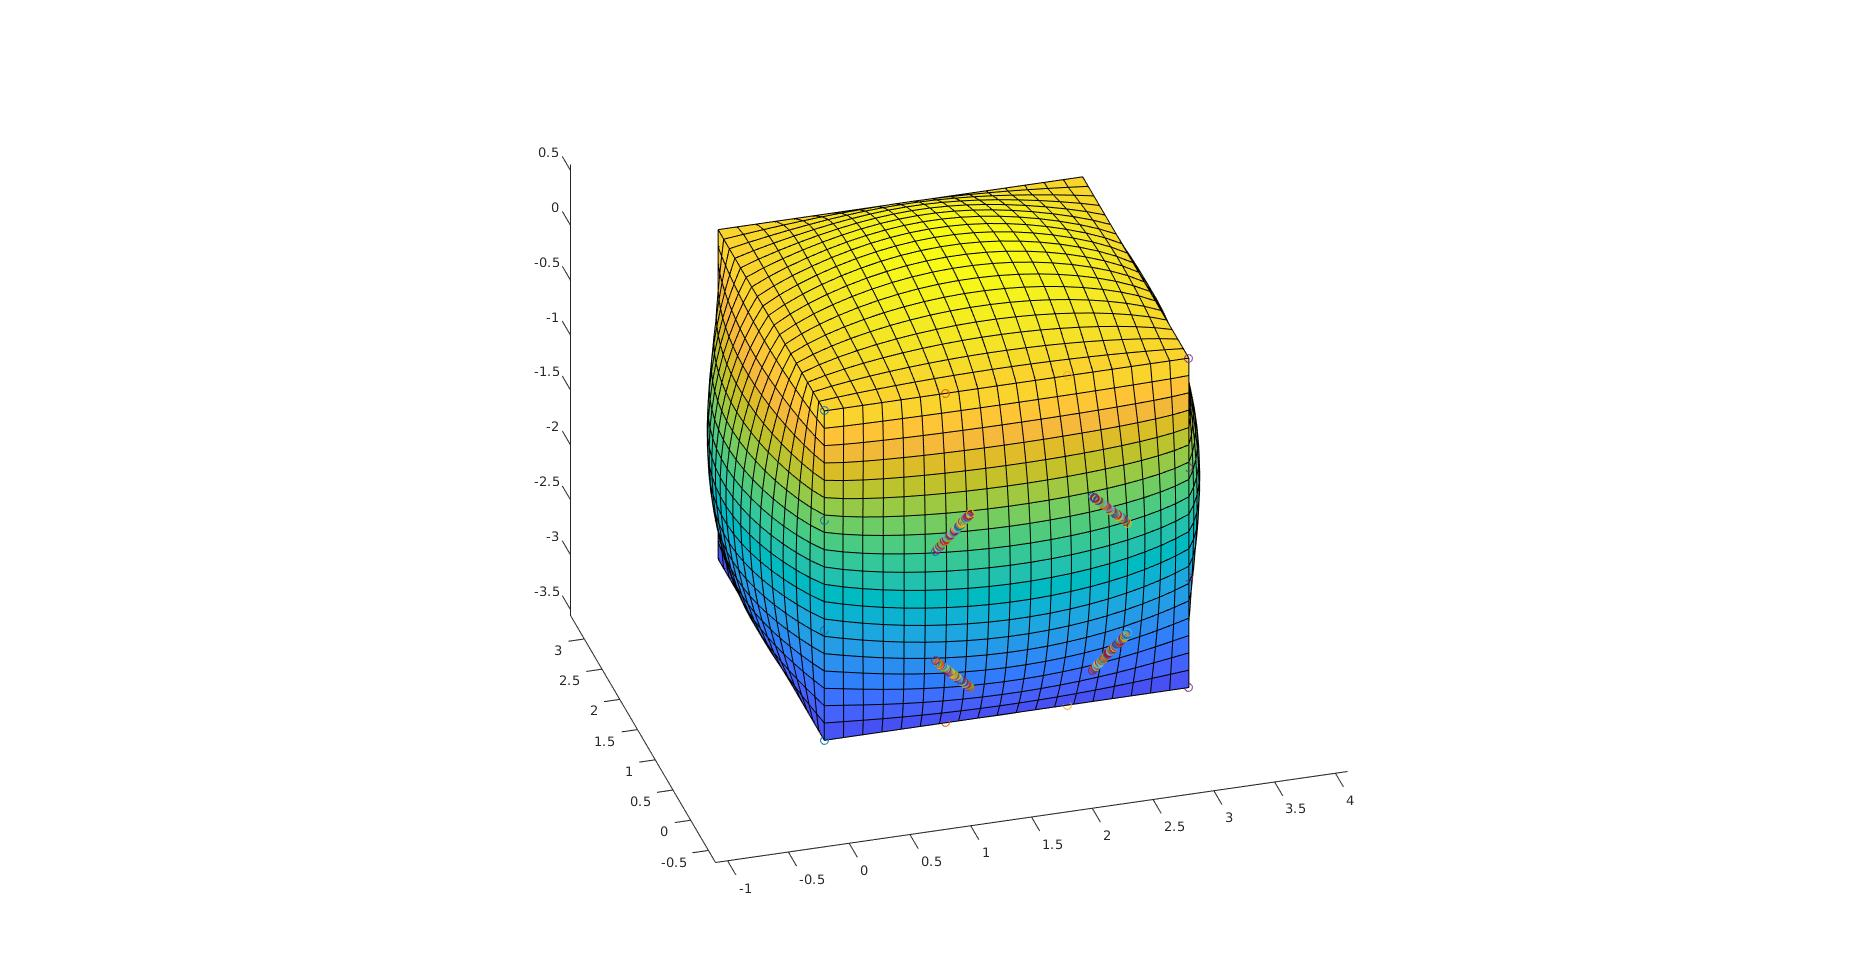
\includegraphics[width=15cm]{gregory_kocka.jpg}
	\caption{Primer Gregoryjeve ideje na kockastem telesu}
	\label{fig:g_kocka}
\end{figure}

% posebna kocka
\begin{figure}[h]
	\centering
	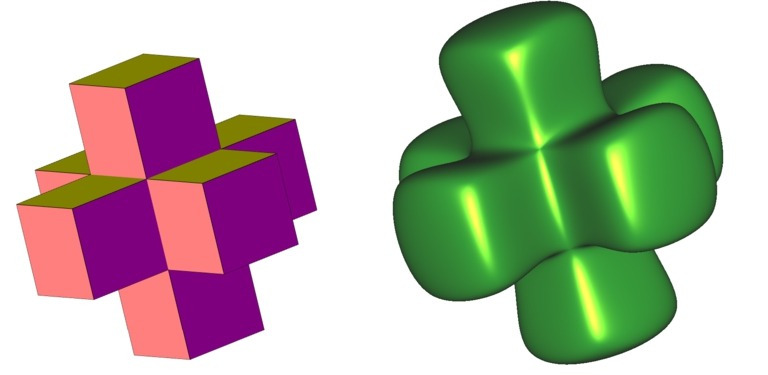
\includegraphics[width=9cm]{posebna_kocka.jpg}
	\caption{Posebna kocka}
\end{figure}

% človeček
\begin{figure}[H]
	\centering
	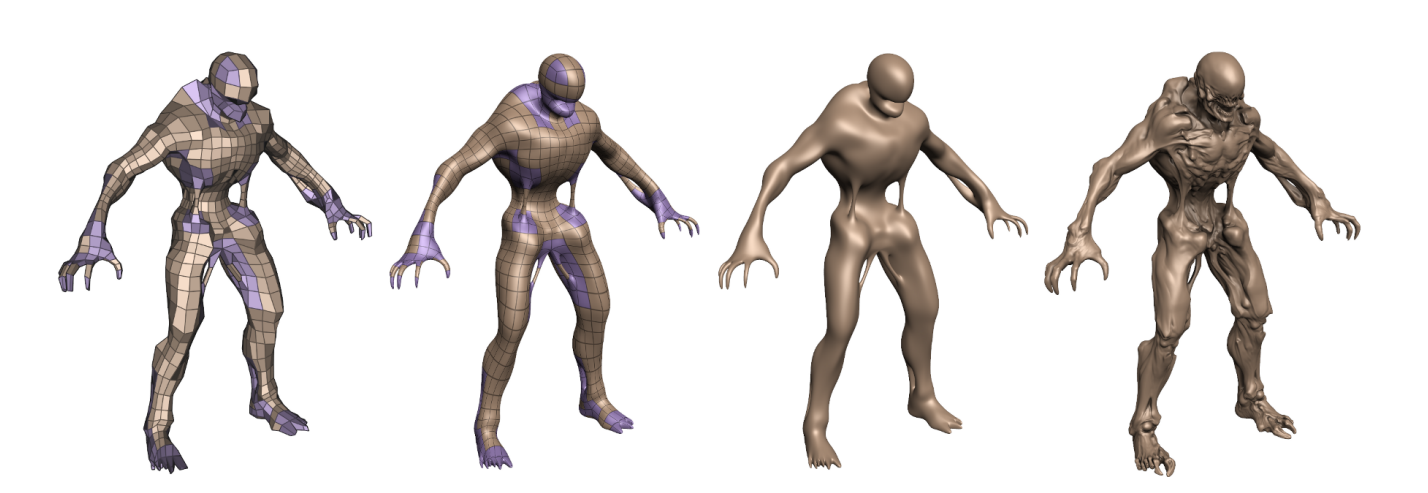
\includegraphics[width=10cm]{koncni_primer.png}
	\caption{Zahtevnejša struktura - človek}
	\label{človek}
\end{figure}

Kot smo že omenili se Gregoryjeve krpe uporabljajo v računalniški grafiki.
Zgoraj sta prikazana še posebna kocka in pa bolj zapletena figura.
Na sliki \ref{človek} je osnovno telo pokrito iz samih štirikotnikov. Na vsakem izmed njih skonstruiramo kvadratno Gregoryjevo krpo. Čisto na desni so nato z displacement map dodane še podrobnosti.

\begin{thebibliography}{99}

%	\bibitem{referenca-clanek}
%	I.~Priimek, \emph{Naslov članka}, okrajšano ime revije \textbf{letnik revije} (leto izida) strani od--do.
	
	\bibitem{osnovni clanek}
	G.~J.~Hettinga, J.~Kosinka: \emph{Multisided generalisations of Gregory patches},
	Computer Aided Geometric Design, \textbf{62}, (2018), 166–180.
	
	\bibitem{dodaten clanek}
	C.~Loop, S.~Schaefer, T.~Ni, I.~Castaño, \emph{Approximating Subdivision Surfaces with Gregory Patches for Hardware Tessellation}, ACM Trans. Graph., \textbf{12}, (2009)
	
\end{thebibliography}






\end{document}